\documentclass[tikz, border=10pt]{standalone}
\usepackage{amsmath, amssymb}
\usetikzlibrary{positioning, calc, shapes.geometric, arrows.meta, patterns}

% Define custom publication-ready colors
\definecolor{PiG_color}{RGB}{0, 120, 0}
\definecolor{stable_blue}{RGB}{31, 119, 180}
\definecolor{unstable_gray}{RGB}{120, 120, 120}
\definecolor{fold_red}{RGB}{214, 39, 40}
\definecolor{amber}{RGB}{255, 191, 0}

\begin{document}

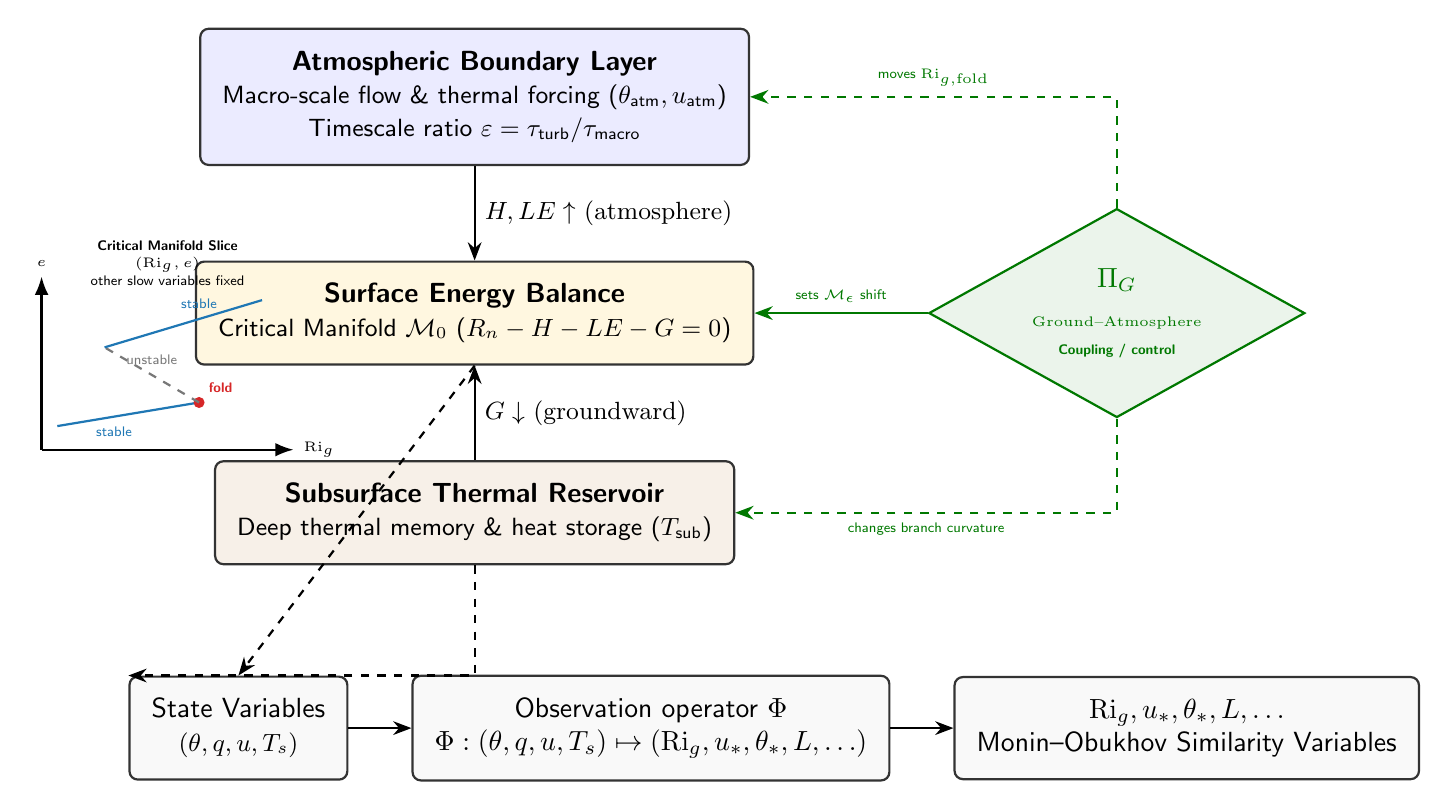
\begin{tikzpicture}[
    >=Stealth,
    node distance=1.2cm and 1.5cm,
    font=\sffamily\small,
    % Standard block styles
    block/.style={
        draw=black!80,
        thick,
        rectangle,
        rounded corners=3pt,
        align=center,
        inner sep=8pt,
        fill=white,
        font=\sffamily
    },
    % Prominent Pi_G diamond style
    pig_diamond/.style={
        draw=PiG_color,
        text=PiG_color,
        shape=diamond,
        aspect=1.8,
        thick,
        align=center,
        inner sep=3pt,
        fill=PiG_color!8,
        font=\sffamily\bfseries
    },
    arrow/.style={->, thick, >=Stealth},
    dashed_arrow/.style={->, thick, >=Stealth, dashed}
]

    % ==========================================
    % 1. PHYSICAL LAYERS & MANIFOLD
    % ==========================================

    % Subsurface Thermal Reservoir (formerly Deep Soil)
    \node (subsurface) [block, fill=brown!12, minimum width=6cm] {
        \textbf{Subsurface Thermal Reservoir} \\
        \small Deep thermal memory \& heat storage ($T_{\text{sub}}$)
    };

    % Surface Energy Balance / Critical Manifold (formerly Skin Layer)
    \node (seb) [block, above=of subsurface, fill=amber!12, minimum width=6cm] {
        \textbf{Surface Energy Balance} \\
        \small Critical Manifold $\mathcal{M}_0$ ($R_n - H - LE - G = 0$)
    };

    % Atmospheric Layer
    \node (atmos) [block, above=of seb, fill=blue!8, minimum width=6cm] {
        \textbf{Atmospheric Boundary Layer} \\
        \small Macro-scale flow \& thermal forcing ($\theta_{\text{atm}}, u_{\text{atm}}$)\\
        \small Timescale ratio $\varepsilon = \tau_{\text{turb}}/\tau_{\text{macro}}$
    };

    % Vertical exchange arrows
    \draw [arrow] (subsurface.north) -- (seb.south) node[midway, right, font=\small] {$G\downarrow$ (groundward)};
    \draw [arrow] (atmos.south) -- (seb.north) node[midway, right, font=\small] {$H, LE\uparrow$ (atmosphere)};

    % ==========================================
    % 2. PROMINENT \Pi_G DIAMOND NODE
    % ==========================================

    \node (pig_box) [pig_diamond, right=2.2cm of seb] {
        $\Pi_G$ \\[2pt]
        \normalfont\tiny Ground--Atmosphere \\[ -2pt]
        \tiny Coupling / control
    };

    % Coupling linkages from \Pi_G
    \draw [arrow, PiG_color] (pig_box.west) -- (seb.east)
        node[midway, above, font=\tiny\sffamily] {sets $\mathcal{M}_\epsilon$ shift};
    \draw [dashed_arrow, PiG_color] (pig_box.north) |- (atmos.east)
        node[near end, above, font=\tiny\sffamily] {moves $\mathrm{Ri}_{g,\mathrm{fold}}$};
    \draw [dashed_arrow, PiG_color] (pig_box.south) |- (subsurface.east)
        node[near end, below, font=\tiny\sffamily] {changes branch curvature};

    % ==========================================
    % 3. FOLD INSET (GSPT CRITICAL MANIFOLD)
    % ==========================================

    \begin{scope}[shift={(-5.5cm, 0.8cm)}]
        \node[font=\tiny\sffamily\bfseries, align=center] at (1.6, 2.45) {Critical Manifold Slice\\$(\mathrm{Ri}_g, e)$};
        \node[font=\tiny\sffamily, align=center] at (1.6, 2.15) {other slow variables fixed};

        \draw[->, thick, -{Latex}] (0,0) -- (3.2,0) node[right, font=\tiny\sffamily] {$\mathrm{Ri}_g$};
        \draw[->, thick, -{Latex}] (0,0) -- (0,2.2) node[above, font=\tiny\sffamily] {$e$};

        % Fold curve geometry
        % Lower stable branch
        \draw[thick, stable_blue] (0.2, 0.3) -- (2.0, 0.6)
            node[pos=0.4, below, font=\tiny\sffamily, text=stable_blue] {stable};

        % Fold point
        \fill[fold_red] (2.0, 0.6) circle (2pt)
            node[above right, font=\tiny\sffamily\bfseries, text=fold_red] {fold};

        % Unstable branch (middle)
        \draw[thick, dashed, unstable_gray] (2.0, 0.6) -- (0.8, 1.3)
            node[pos=0.5, above, font=\tiny\sffamily, text=unstable_gray] {unstable};

        % Upper stable branch
        \draw[thick, stable_blue] (0.8, 1.3) -- (2.8, 1.9)
            node[pos=0.6, above, font=\tiny\sffamily, text=stable_blue] {stable};
    \end{scope}

    % ==========================================
    % 4. OBSERVATION CHAIN (STATE TO METRICS)
    % ==========================================

    \node (obs_state) [block, below=1.4cm of subsurface, xshift=-3cm, fill=gray!5] {
        State Variables \\
        \small $(\theta, q, u, T_s)$
    };

    \node (obs_operator) [block, right=0.8cm of obs_state, fill=gray!5] {
        Observation operator $\Phi$\\
        $\Phi:(\theta, q, u, T_s) \mapsto (\mathrm{Ri}_g, u_*, \theta_*, L, \ldots)$
    };

    \node (obs_metrics) [block, right=0.8cm of obs_operator, fill=gray!5] {
        $\mathrm{Ri}_g, u_*, \theta_*, L, \ldots$\\
        Monin--Obukhov Similarity Variables
    };

    % Flow arrows for observation operator framework
    \draw [arrow] (obs_state.east) -- (obs_operator.west);
    \draw [arrow] (obs_operator.east) -- (obs_metrics.west);
    \draw [dashed_arrow] (subsurface.south) |- (obs_state.north west);
    \draw [dashed_arrow] (seb.south) -- (obs_state.north);

\end{tikzpicture}

\end{document}